% Multi-Modal CVD Poster (24x36 in, landscape)
\documentclass[final]{beamer}

% ---------- PACKAGES ----------
\usepackage[size=custom,width=91.4,height=61.0,scale=1.00]{beamerposter} % 36x24 in, reduced scale for fitting content
\usepackage[T1]{fontenc}
\usepackage{lmodern}
\usepackage{graphicx}
\usepackage{booktabs}
\usepackage{amsmath,amssymb}
\usepackage{wrapfig}
\usepackage{qrcode}
\usepackage{url}
\usepackage{enumitem}
\usepackage{microtype}

% Search image paths one level up from Report/ (root `figures/` and `results/`)
\graphicspath{{../figures/}{../results/}{./}}

% ---------- UF COLORS ----------
\definecolor{UFBlue}{HTML}{0021A5}
\definecolor{UFOrange}{HTML}{FA4616}
\definecolor{UFGray}{HTML}{F5F5F5}

\setbeamercolor{background canvas}{bg=white}
\setbeamercolor{block title}{fg=white,bg=UFBlue}
\setbeamercolor{block body}{bg=UFGray,fg=black}
\setbeamercolor{title}{fg=UFBlue}
\setbeamercolor{frametitle}{fg=UFBlue}

\setbeamertemplate{itemize item}{\color{UFBlue}$\blacktriangleright$}
\setbeamertemplate{itemize subitem}{\color{UFOrange}\scriptsize$\bullet$}

% Compact lists and slightly smaller block body font to improve fit on the poster
\usepackage{enumitem}
\setlist[itemize]{nosep, topsep=0.2em, leftmargin=1.1em}
\setbeamerfont{block body}{size=\small}
\setbeamerfont{block title}{size=\large}
\setbeamerfont{title}{size=\Huge}
\setlength{\columnsep}{1.2em}

% ---------- TITLE ----------
\title{\textbf{Multi-Modal Predictors for Cardiovascular Disease Risk and Outcomes}}
\author{\textbf{Angel Morenu}}
\institute{University of Florida \quad|\quad EEE 6778 -- Applied Machine Learning II}

% ---------- BEGIN DOCUMENT ----------
\begin{document}
\begin{frame}[t]

% ============================================================
% COLUMN LAYOUT (3 columns)
% ============================================================
\begin{columns}[t,totalwidth=\textwidth]

% ============================================================
% COLUMN 1
% ============================================================
\begin{column}{0.32\textwidth}

% ----- TITLE & ABSTRACT -----
\begin{block}{Project Overview}
\large
\textbf{Goal.} Build a multi-modal system that fuses:
\begin{itemize}[leftmargin=1.1em]
  \item demographic \& clinical tabular data,
  \item hospital admission information, and
  \item raw ECG signals
\end{itemize}
to estimate cardiovascular disease (CVD) risk and support future edge deployment.

\vspace{0.4em}
\textbf{Contributions (Deliverable 3).}
\begin{itemize}[leftmargin=1.1em]
  \item Stabilized preprocessing and training for tabular and ECG streams.
  \item Added a robust evaluation harness with calibration and performance dashboards.
  \item Enhanced a Streamlit UI with explanations and JSONL logging.
  \item Integrated SHAP-style and ECG saliency visualizations for interpretability.
\end{itemize}
\end{block}

% ----- PROBLEM & MOTIVATION -----
\begin{block}{Problem \& Motivation}
\textbf{Clinical need.}
CVD remains a leading global cause of death. Risk scores are often based only on tabular factors (age, BP, cholesterol) and ignore rich signal data from ECGs.

\textbf{Challenge.}
\begin{itemize}[leftmargin=1.1em]
  \item Heterogeneous data (structured + time series).
  \item Small, imbalanced datasets.
  \item Need for interpretable predictions to support clinical trust.
\end{itemize}

\textbf{Vision.}
A modular, reproducible pipeline that can eventually power:
\begin{itemize}[leftmargin=1.1em]
  \item point-of-care risk triage tools, and
  \item lightweight edge deployments (e.g., wearable sensors).
\end{itemize}
\end{block}

% ----- DATASETS -----
\begin{block}{Data Sources}
\textbf{Tabular (CVD Risk).}
\begin{itemize}[leftmargin=1.1em]
  \item Kaggle Cardiovascular Disease dataset:
  \item Demographics: age, sex, BMI, blood pressure, cholesterol, smoking.
\end{itemize}

\textbf{Hospital / Clinical.}
\begin{itemize}[leftmargin=1.1em]
  \item Admission indicators and simplified comorbidities.
\end{itemize}

\textbf{ECG Signals.}
\begin{itemize}[leftmargin=1.1em]
  \item Single-lead ECG segments (PTB-XL-inspired pipeline).
  \item Resampled, filtered, and padded/truncated to 2000 time steps.
\end{itemize}

\textbf{Preprocessing Highlights.}
\begin{itemize}[leftmargin=1.1em]
  \item scikit-learn \texttt{ColumnTransformer} for impute/scale/encode \cite{pedregosa2011scikit}.
  \item Defensive alignment: if split sizes disagree, arrays are truncated to a safe common length with warnings.
\end{itemize}
\vspace{0.4em}
	extbf{Reproducibility artifacts.} See the repository (\texttt{artifacts/}, \texttt{scripts/}) for model checkpoints and reproduction scripts.
\end{block}

\end{column}

% ============================================================
% COLUMN 2
% ============================================================
\begin{column}{0.36\textwidth}

% ----- ARCHITECTURE DIAGRAM -----
\begin{block}{System Architecture}
\begin{center}
% Include architecture figure if present under ../figures/, otherwise show a small placeholder box
\IfFileExists{../figures/multimodal_cvd_architecture.png}{%
  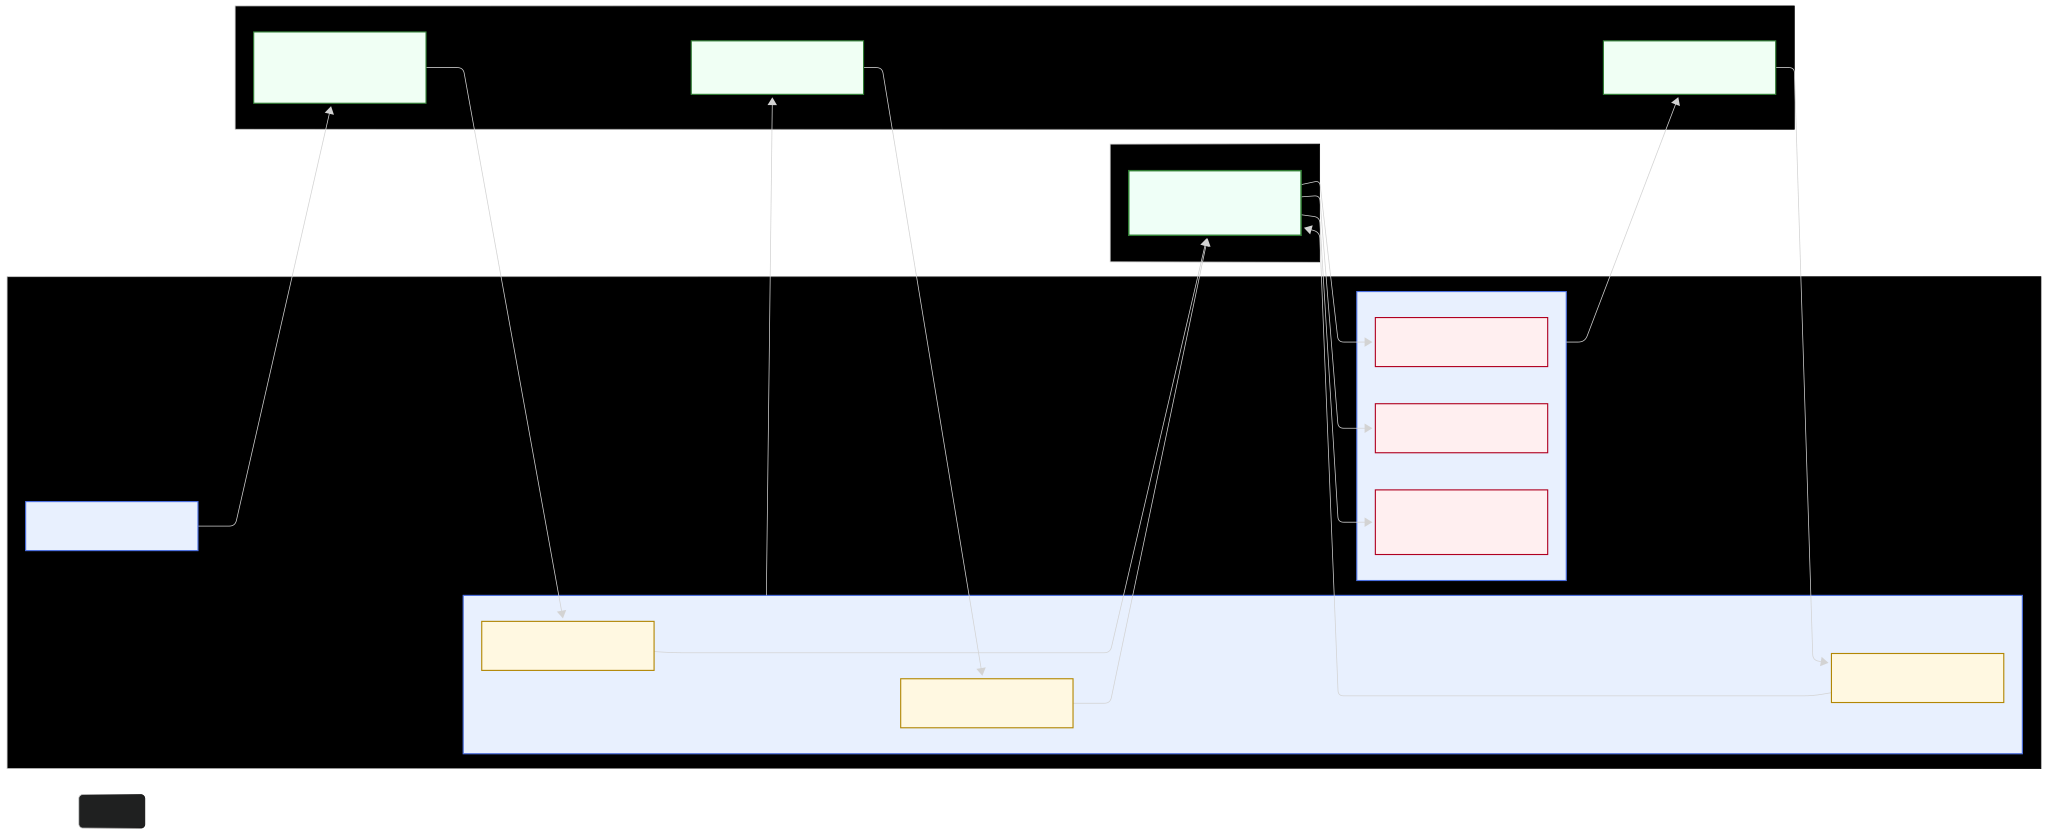
\includegraphics[width=\linewidth]{../figures/multimodal_cvd_architecture.png}%
}{%
  \fbox{Missing: ../figures/multimodal_cvd_architecture.png}%
}
\end{center}
\vspace{-0.4em}
\small
The pipeline fuses preprocessed tabular features, clinical context, and CNN-based ECG embeddings into a PyTorch fusion classifier \cite{paszke2019pytorch}. Baseline models (LogReg, RF, GBM) support ablations and calibration.
\end{block}

% ----- MODELING APPROACH -----
\begin{block}{Modeling \& Fusion}
\textbf{Tabular Branch.}
\begin{itemize}[leftmargin=1.1em]
  \item Baselines: Logistic Regression, Random Forest.
  \item Features: age, blood pressure, cholesterol, lifestyle, admissions.
\end{itemize}

\textbf{ECG Branch.}
\begin{itemize}[leftmargin=1.1em]
  \item 1D CNN feature extractor (with optional LSTM head).
  \item Trained to learn temporal patterns from 2000-sample windows.
\end{itemize}

\textbf{Fusion Head.}
\begin{itemize}[leftmargin=1.1em]
  \item Concatenate tabular embedding + ECG embedding.
  \item Dense layers + dropout + sigmoid output.
  \item Fallback: stacked logistic regression over unimodal predictions when checkpoints are unavailable.
\end{itemize}
\end{block}

% ----- RESULTS TABLE -----
\begin{block}{Quantitative Results (Held-out Snapshot)}
\small
\begin{center}
\begin{tabular}{lccc}
\toprule
Metric & Tabular & ECG & Fusion \\
\midrule
Accuracy     & 0.571 & 0.438 & 0.563 \\
ROC AUC      & 0.527 & 0.297 & 0.453 \\
PR AUC       & 0.560 & 0.375 & 0.526 \\
Brier Score  & 0.351 & 0.331 & 0.362 \\
F1 Score     & 0.609 & 0.526 & 0.588 \\
Sensitivity  & 0.700 & 0.625 & 0.625 \\
Specificity  & 0.455 & 0.250 & 0.500 \\
\bottomrule
\end{tabular}
\end{center}
\vspace{0.6em}
\footnotesize
Summary: the fusion model improves over unimodal baselines on several thresholds in this snapshot, but absolute scores are limited by dataset size and class imbalance. A quick Platt-scaling calibrator was fitted from available held-out predictions; see \texttt{artifacts/calibrator.joblib} and \texttt{results/calibration\_summary.json} for details.
\vspace{0.4em}
Metrics are computed from per-run prediction artifacts using a reproducible evaluation harness (\texttt{generate\_predictions.py}, \texttt{metric\_summary.json}). The focus in Deliverable~3 is stability and interpretability rather than maximizing AUC.
\end{block}

% ----- PERFORMANCE DASHBOARD -----
\begin{block}{Performance Dashboard (Fusion)}
\begin{center}
\IfFileExists{../figures/perf_dashboard_fusion.png}{%
  \includegraphics[width=0.95\linewidth]{../figures/perf_dashboard_fusion.png}%
}{%
  \fbox{Missing: ../figures/perf_dashboard_fusion.png}%
}
\end{center}
\footnotesize
Dashboard summarizing ROC, PR curve, confusion matrix, and probability histogram for the fusion model. Scripts automatically regenerate this figure from saved predictions.
\end{block}

\end{column}

% ============================================================
% COLUMN 3
% ============================================================
\begin{column}{0.32\textwidth}

% ----- CALIBRATION & CONFUSION -----
\begin{block}{Calibration \& Error Patterns}
\begin{center}
\IfFileExists{../figures/calibration_curve_fusion.png}{%
  \includegraphics[width=0.95\linewidth]{../figures/calibration_curve_fusion.png}%
}{%
  \fbox{Missing: ../figures/calibration_curve_fusion.png}%
}
\\[0.5em]
\IfFileExists{../figures/confusion_matrix.png}{%
  \includegraphics[width=0.7\linewidth]{../figures/confusion_matrix.png}%
}{%
  \fbox{Missing: ../figures/confusion_matrix.png}%
}
\end{center}
\footnotesize
Calibration reveals over- and under-confidence across bins; the confusion matrix highlights a tendency to over-predict the positive class. These diagnostics motivated future work on temperature scaling and subgroup calibration. A quick Platt-scaling calibrator was trained as a proof-of-concept and saved to \texttt{artifacts/calibrator.joblib}; with the small validation subset used here, calibration changes were modest (see \texttt{results/calibration\_summary.json}).
\end{block}

% ----- INTERPRETABILITY -----
\begin{block}{Interpretability: SHAP \& ECG Saliency}
\begin{center}
% SHAP (left) and ECG saliency (right) — use ../figures/ and fallback boxes if missing
\IfFileExists{../figures/shap_force_example.png}{%
  \includegraphics[width=0.48\linewidth]{../figures/shap_force_example.png}%
}{%
  \fbox{Missing: ../figures/shap_force_example.png}%
}
\hfill
\IfFileExists{../figures/ecg_saliency.png}{%
  \includegraphics[width=0.48\linewidth]{../figures/ecg_saliency.png}%
}{%
  \fbox{Missing: ../figures/ecg_saliency.png}%
}
\end{center}
\footnotesize
Left: SHAP-style values (or leave-one-out importance fallback) summarizing feature contributions to a single prediction. Right: ECG saliency (gradient-based) overlay highlighting time regions most influential for the CNN embedding. Both explainers are produced by scripts in \texttt{scripts/}: \texttt{run\_shap\_tabular.py} and \texttt{make\_ecg\_saliency.py} and are shown as examples for human-in-the-loop review. SHAP requires the optional \texttt{shap} package; a computationally cheaper leave-one-out fallback is implemented if it is unavailable.
\end{block}

% ----- UI / HCI -----
\begin{block}{Streamlit UI \& HCI Design}
\begin{center}
\IfFileExists{../figures/ui_demo.png}{%
  \includegraphics[width=0.95\linewidth]{../figures/ui_demo.png}%
}{%
  \fbox{Missing: ../figures/ui_demo.png}%
}
\end{center}
\footnotesize
The Streamlit demo integrates:
\begin{itemize}[leftmargin=1.1em]
  \item Tabular form inputs for key risk factors.
  \item ECG file upload and visualization.
  \item Risk probability with color-coded guidance.
  \item An \emph{Explanations} expander showing SHAP and saliency figures.
  \item JSONL logging of every prediction for future audits.
\end{itemize}
The interface is designed for clarity, accessibility, and future extension to edge or clinical prototypes.
\end{block}

% ----- RESPONSIBLE AI & FUTURE WORK -----
\begin{block}{Responsible AI \& Next Steps}
\textbf{Responsible AI Actions.}
\begin{itemize}[leftmargin=1.1em]
  \item Transparent explanations (SHAP + saliency) in the UI.
  \item Local-only logging and de-identified demo inputs.
  \item Explicit documentation of limitations and failure modes.
\end{itemize}

\textbf{Planned Extensions.}
\begin{itemize}[leftmargin=1.1em]
  \item Calibration (temperature scaling, isotonic regression).
  \item Subgroup fairness analysis by age/sex/race.
  \item Model compression (pruning / distillation) for edge devices.
  \item Expanded datasets and cross-validated hyperparameter tuning.
\end{itemize}
\vspace{0.6em}
	extbf{Limitations.} Small validation sets and pickled transformer versioning can limit reproducibility; see the README for mitigation.
\vspace{0.6em}
	extbf{Immediate Next Steps for Reproducibility.} Commit and document model artifacts and expand held-out evaluation folds for robust calibration and reliability testing.
\end{block}

% Artifacts & scripts listed in README and repository; removed detailed block to improve layout and avoid overflow.

% ----- QR CODE / CONTACT -----
\begin{block}{Code, Demo \& Contact}
\begin{columns}[T,totalwidth=\linewidth]
\begin{column}{0.55\linewidth}
\small
\textbf{GitHub Repository}\\
\url{https://github.com/angelmorenu/multi-modal-cvd-predictor}

\vspace{0.5em}
\textbf{Contact}\\
Angel Morenu \\
\texttt{angel.morenu@ufl.edu}
\end{column}
\begin{column}{0.45\linewidth}
\centering
% QR code generation can be fragile in some TeX setups; use a placeholder box instead
\fbox{QR code: see repo}\\
\footnotesize Scan for code, README, and reproduction instructions.
\end{column}
\end{columns}
\end{block}

\end{column}

\end{columns}

% References strip removed for debugging; add references if needed later.

\end{frame}
\end{document}
